%iffalse
\let\negmedspace\undefined
\let\negthickspace\undefined
\documentclass[journal,12pt,onecolumn]{IEEEtran}
\usepackage{cite}
\usepackage{amsmath,amssymb,amsfonts,amsthm}
\usepackage{algorithmic}
\usepackage{graphicx}
\usepackage{textcomp}
\usepackage{xcolor}
\usepackage{txfonts}
\usepackage{listings}
\usepackage{enumitem}
\usepackage{mathtools}
\usepackage{gensymb}
\usepackage{comment}
\usepackage[breaklinks=true]{hyperref}
\usepackage{tkz-euclide} 
\usepackage{listings}
\usepackage{gvv}                                        
%\def\inputGnumericTable{}                                 
\usepackage[latin1]{inputenc}                                
\usepackage{color}                                            
\usepackage{array}                                            
\usepackage{longtable}                                       
\usepackage{calc}                                             
\usepackage{multirow}                                         
\usepackage{hhline}                                           
\usepackage{ifthen}                                           
\usepackage{lscape}
\usepackage{tabularx}
\usepackage{array}
\usepackage{float}

\usepackage{enumitem}
\usepackage{xcolor}
%\usepackage{multicol}


\newtheorem{theorem}{Theorem}[section]
\newtheorem{problem}{Problem}
\newtheorem{proposition}{Proposition}[section]
\newtheorem{lemma}{Lemma}[section]
\newtheorem{corollary}[theorem]{Corollary}
\newtheorem{example}{Example}[section]
\newtheorem{definition}[problem]{Definition}
\newcommand{\BEQA}{\begin{eqnarray}}
\newcommand{\EEQA}{\end{eqnarray}}
\newcommand{\define}{\stackrel{\triangle}{=}}
\theoremstyle{remark}
\newtheorem{rem}{Remark}

\title{1.7.4}
\author{AI24BTECH11023 - Tarun Reddy Pakala}
\begin{document}
\bibliographystyle{IEEEtran}

\maketitle
\bigskip

\renewcommand{\thefigure}{\theenumi}
\renewcommand{\thetable}{\theenumi}


\textbf{Question}:\\
Using vectors, prove that the points \brak{2,-1,3},\brak{3,-5,1} and \brak{-1,11,9} are collinear.\\
\solution\\
\\

Next, we construct the matrix using these vectors:

\[
\text{Matrix} = 
\begin{pmatrix}
\overrightarrow{B-A} & \overrightarrow{C-A}
\end{pmatrix}
= 
\begin{pmatrix}
1 & -3 \\
-4 & 12 \\
-2 & 6
\end{pmatrix}
\]

Now, we perform row reduction:

\[
\begin{pmatrix}
1 & -3 \\
-4 & 12 \\
-2 & 6
\end{pmatrix}
\rightarrow
\begin{pmatrix}
1 & -3 \\
0 & 0 \\
0 & 0
\end{pmatrix}
\]

Since the matrix has rank 1 (only one non-zero row), the points are collinear.


\title{Figure on New Page Example}
\author{}
\date{}
\maketitle

% Some introductory text


\newpage % Start a new page before the figure

\begin{figure}[h]
    \centering
    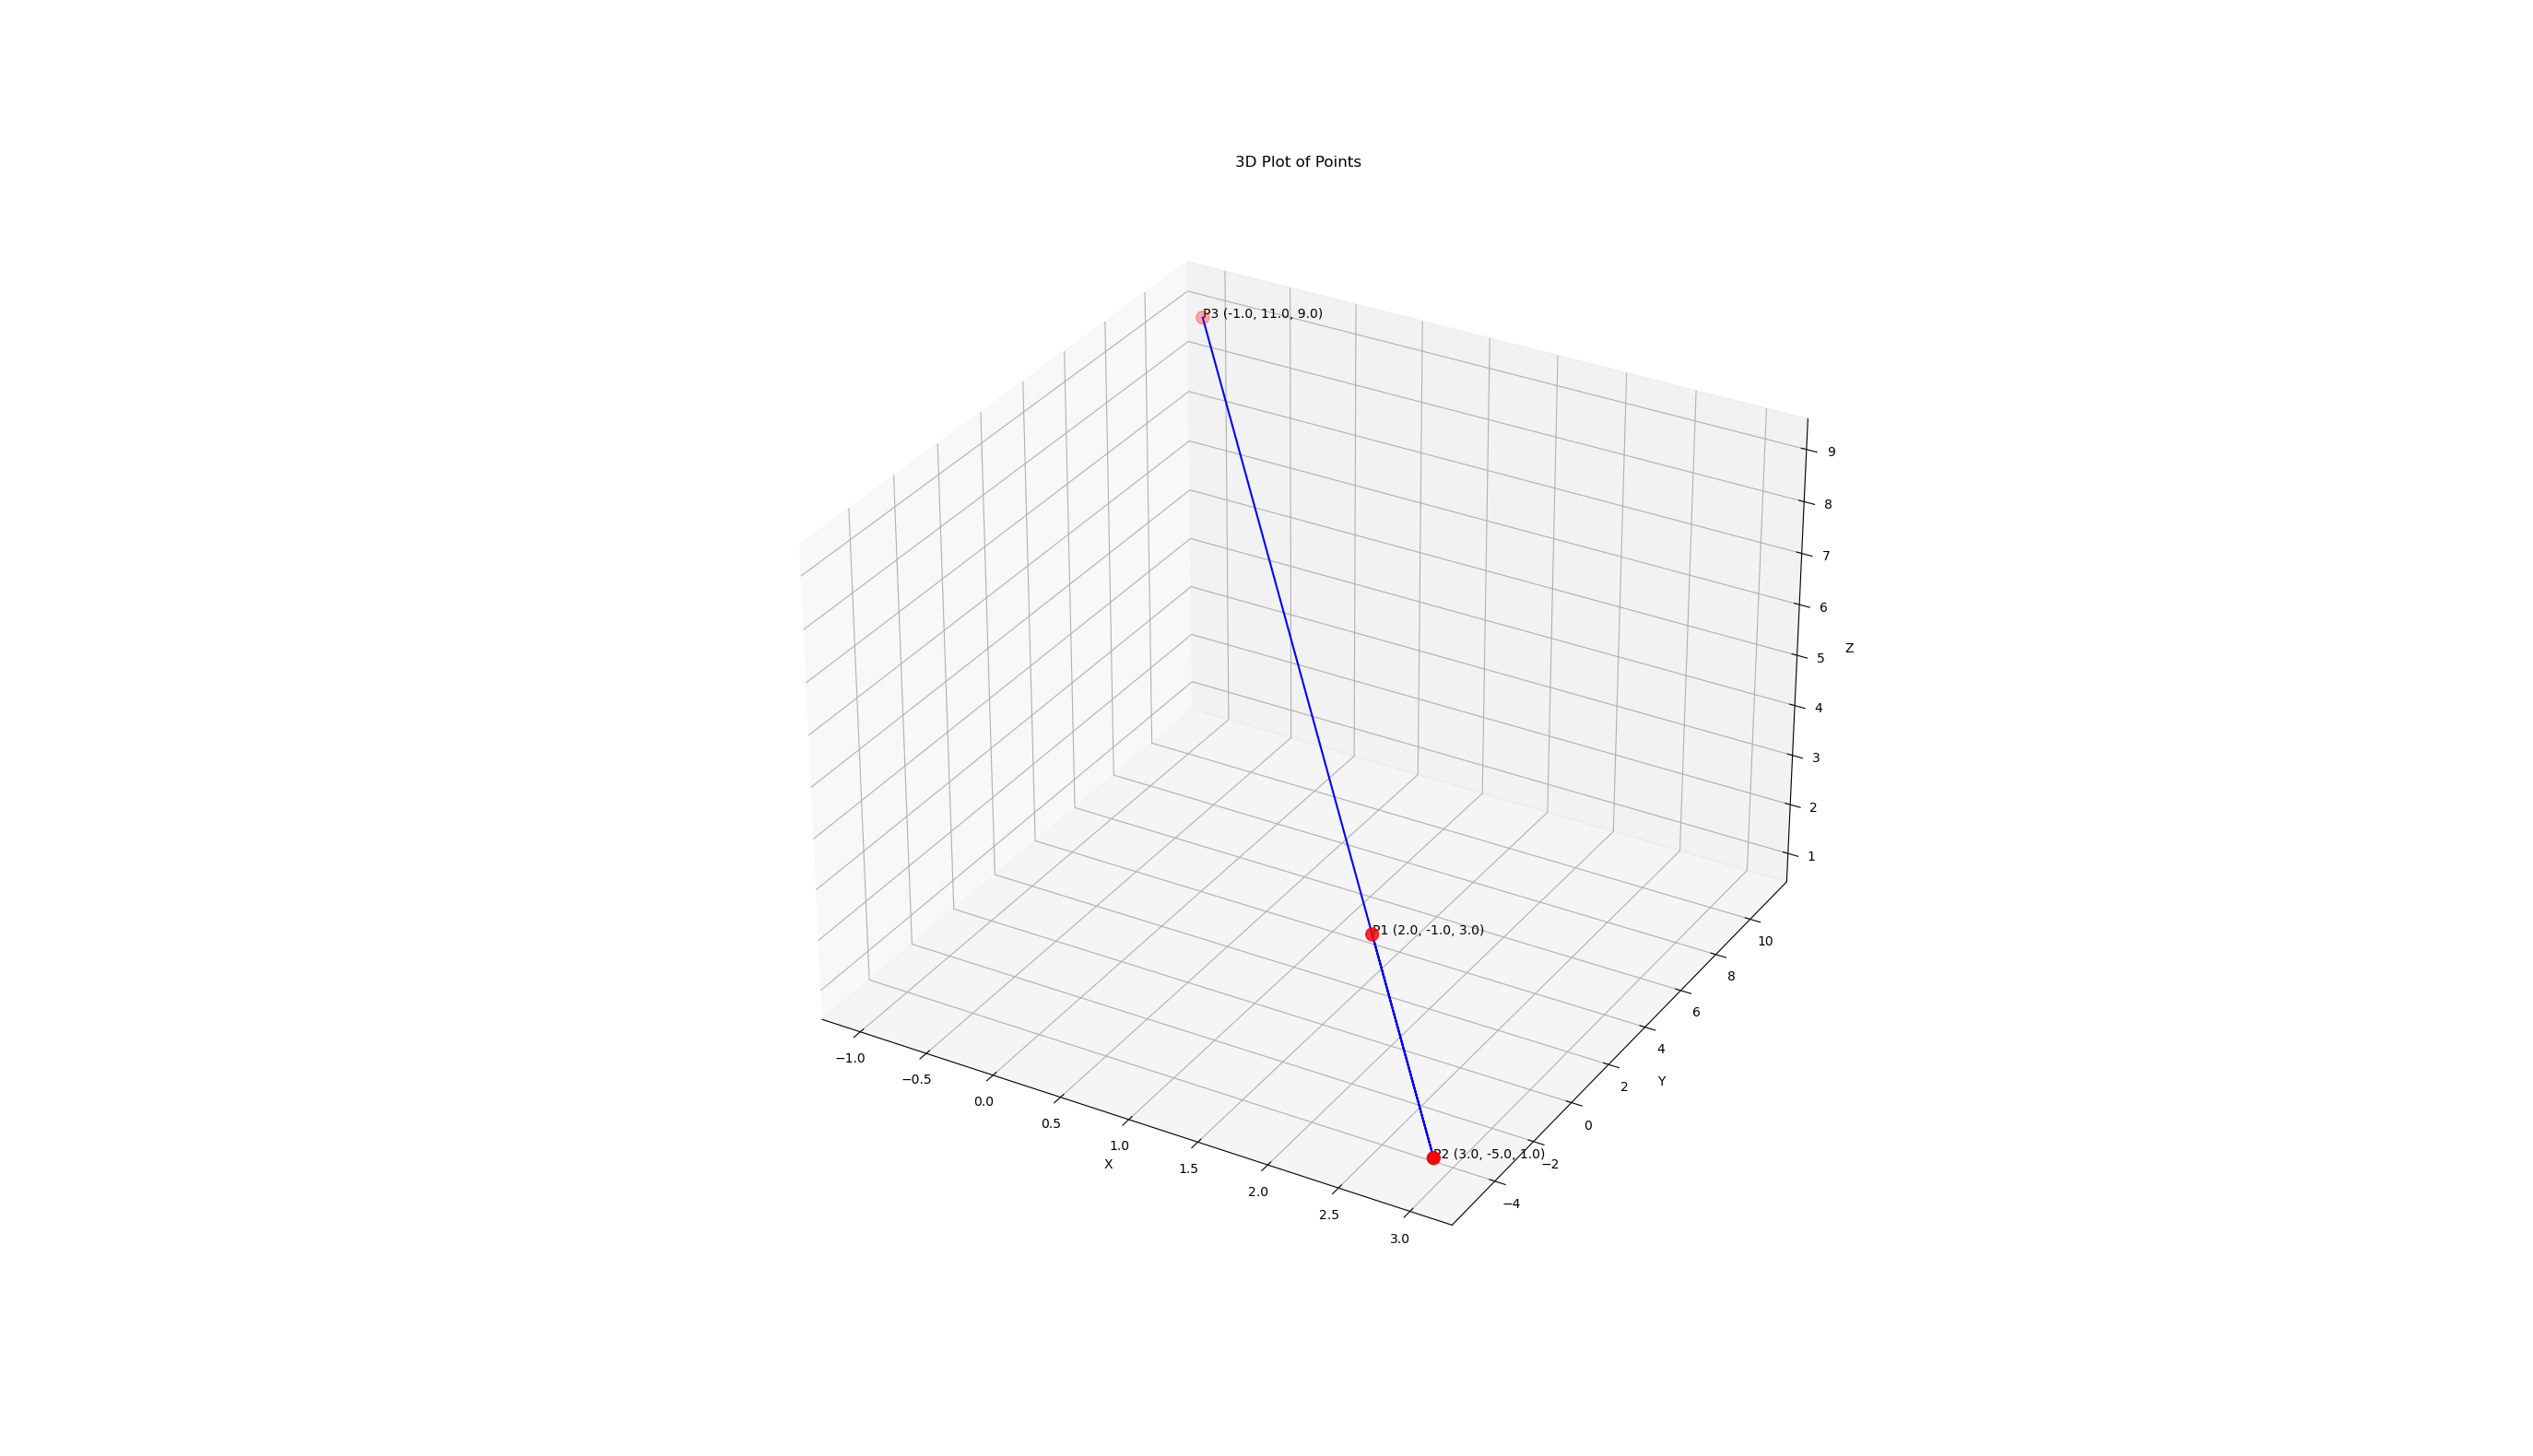
\includegraphics[width=\textwidth]{figure.png} 
    \label{fig:example_image}
\end{figure}

\end{document}


